%%
%%
%%


%-------------------- begin preamble ----------------------

\documentclass[%
oneside,                 % oneside: electronic viewing, twoside: printing
final,                   % draft: marks overfull hboxes, figures with paths
10pt]{article}

\listfiles               %  print all files needed to compile this document

\usepackage{relsize,makeidx,color,setspace,amsmath,amsfonts,amssymb}
\usepackage[table]{xcolor}
\usepackage{bm,ltablex,microtype}
\usepackage{float}
\usepackage[pdftex]{graphicx}
\usepackage{graphicx}



\usepackage{fancyvrb} % packages needed for verbatim environments

\usepackage[T1]{fontenc}
%\usepackage[latin1]{inputenc}
\usepackage{ucs}
\usepackage[utf8x]{inputenc}

\usepackage{lmodern}         % Latin Modern fonts derived from Computer Modern

% Hyperlinks in PDF:
\definecolor{linkcolor}{rgb}{0,0,0.4}
\usepackage{hyperref}
\hypersetup{
    breaklinks=true,
    colorlinks=true,
    linkcolor=linkcolor,
    urlcolor=linkcolor,
    citecolor=black,
    filecolor=black,
    pdfmenubar=true,
    pdftoolbar=true,
    bookmarksdepth=3   % Uncomment (and tweak) for PDF bookmarks with more levels than the TOC
    }
%\hyperbaseurl{}   % hyperlinks are relative to this root

\setcounter{tocdepth}{2}  % levels in table of contents

% --- fancyhdr package for fancy headers ---
\usepackage{fancyhdr}
\fancyhf{} % sets both header and footer to nothing
\renewcommand{\headrulewidth}{0pt}

\fancypagestyle{plain}{
  \fancyhf{}

%  \renewcommand{\footrulewidth}{0mm}
  \renewcommand{\headrulewidth}{0mm}
}
% Ensure copyright on titlepages with \thispagestyle{empty}
\fancypagestyle{empty}{
  \fancyhf{}

  \renewcommand{\headrulewidth}{0mm}
}

\pagestyle{fancy}

\renewcommand{\figurename}{Figur}
\renewcommand{\tablename}{Tabell}
\renewcommand{\contentsname}{Innholdsfortegnelse}

% prevent orhpans and widows
\clubpenalty = 10000
\widowpenalty = 10000

% --- end of standard preamble for documents ---


% insert custom LaTeX commands...

\raggedbottom
\makeindex
\usepackage[totoc]{idxlayout}   % for index in the toc
\usepackage[nottoc]{tocbibind}  % for references/bibliography in the toc

%-------------------- end preamble ----------------------

\begin{document}

% matching end for #ifdef PREAMBLE

\newcommand{\exercisesection}[1]{\subsection*{#1}}


% ------------------- main content ----------------------



% ----------------- title -------------------------

\thispagestyle{empty}

\begin{center}
{\LARGE\bf
\begin{spacing}{1.25}
Project 3 - Computational physics - FYS3150
\end{spacing}
}
\end{center}

% ----------------- author(s) -------------------------


    \begin{center}
% List of all institutions:
\centerline{{\small Department of Physics, University of Oslo, Norway.}}
\centerline{Philip Niane og Rohullah Akbari}

Link til githubmappen: https://github.com/philipkarim/Philip-and-Rohullah-ComFys
\end{center}

% ----------------- end author(s) -------------------------



\vspace{1cm}

\noindent\textbf{\Large{Abstrakt}}\newline
I denne rapporten...

\tableofcontents
\section{Introduksjon}
Målet med dette prosjektet er å løse er å integrere ved bruk av forskjellige numeriske metoder. De numeriske metodene skal naturligvis programmeres og sammenliknes. Integralet som skal løses er integralet som gir grunntilstandsenergien mellom to elektroner i et helium atom:

\begin{equation}
  \langle \frac{1}{\left| {r}_1 - {r}_2 \right|} \rangle = \int_{-\infty}^{\infty} dr_1dr_2 e^{-2\alpha(r_1, r_2)} \frac{1}{\left| {r}_1 - {r}_2 \right|}
\end{equation}
\noindent Hvor
\begin{equation}
	{\bf r}_i =  x_i {\bf e}_x + y_i {\bf e}_y +z_i {\bf e}_z
\end{equation}
\noindent Som gir
\begin{equation}
	r_i = \sqrt{x_i^2+y_i^2+z_i^2}.
\end{equation}
\noindent Konstanten $\alpha$ blir satt til å være lik 2, da dette tilsvarer ladningen til et helium atom, Z=2.\\
\noindent Metodene som skal ses på i dette prosjektet er Gauss Legendre, Gauss Laguerre og Flere versjoner av Monte Carlo integrasjon. Det blir brukt både kartesiske koordinater og kule koordinater.  Prosjektet gir også trening i bruk av paralellisering av kode som gir programmer som kjøres enda raskere.[3]

\section{Teori}

\subsection{Gauss Kvadratur}
\noindent En av integrasjonsmetodene som skal brukes er Gauss kvadratur. Denne metoden skiller seg ut fra en del andre metoder innenfor numeriske metoder ved at steglengden mellom $x_i$ og $x_{i+1}$ ikke er fast. Gauss kvadratur går ut på å skrive om integranden til følgende form:

\begin{equation}
	A=\int_a^b f(x)dx=\int_a^b W(x)g(x)dx \approx \sum_{i = 0}^{N-1} \omega_i g(x_i)
\end{equation}

\noindent Hvor W(x) er vektfunksjonen, samtidig som aproksimasjonen blir nøyaktig om graden til polynomfunksjonen g(x) er mindre enn 2N-1. Vektene $w_i$ fås gjennom de ortogonale polynoms-algoritmene som for eksempel Legendre, Laguerre, Hermite og Chebyshev. I dette prosjektet fokuseres det kun på Legendre og Laguerre. [1]
\subsubsection{Gauss Legendre Kvadratur}
\noindent Gauss Legendre metode bruker finite integrasjonsgrenser. Vektfunksjonen til Legendres metode W(x)=1, derfor er det mulig ut ifra likning (4) å se at metoden kan kjøres på integralet uten å måtte skrives om. Da $x_i, y_i$ og $z_i$ defineres fra $-\infty$ til $\infty$ vil passende finite grenser settes senere i rapporten.

\subsubsection{Gauss Laguerre Kvadratur}
\noindent Gauss Laguerre metode er fin å bruke når det opereres med grenser som går mot uendelig. Dette passer bra med tanke på at en endring til sfæriske koordinater vil gi r $\in$ [0,$\infty$). Samtidig blir vinkelgrensene $\theta \in$[0,$\pi$] og $\phi \in$[0,$2\pi$].\\
\noindent Laguerre har en vektet funksjon på følgende form: $W(x) = x^{\alpha} e^{-x}$. Dette betyr at integralet som skal utregnes må skrives om på følgende form:

\begin{equation}
  \notag A =
  \int_0^\infty x^\alpha e^{-x} g(x) \, dx = \sum^{N}_{i=1} \omega_ig(x_i).
\end{equation}

\noindent Etter uttrykket er skrevet om til kulekoordinater og skrevet om til formen over, kan uttrykket skrives på følgende måte: (Utledning kan ses i appendix)
\begin{equation*}
    A=\frac{1}{(2\alpha)^5} \int_{0}^\infty\int_0^\infty\int_0^{\pi}\int_0^\pi\int_0^{2\pi}\int_0^{2\pi}W(u_1)W(u_2)g(u, \theta, \phi)\,du_1du_2d\theta_1d\theta_2d\phi_1d\phi_2
\end{equation*}

\noindent Hvor
\begin{equation}
    W(u_i)=(u_i)^2 e^{-u_i}
\end{equation}
\noindent og
\begin{equation}
    g(u_1, u_2, \theta_1, \theta_2, \phi_1, \phi_2) = \frac{\sin \theta_1 \sin \theta_2}{r_{12}}
\end{equation}

\noindent $r_{12}$ og $cos(\beta)$ er oppgitt i oppgaven som:
\begin{equation}
	\frac{1}{r_{12}}= \frac{1}{\sqrt{r_1^2+r_2^2-2r_1r_2\cos(\beta)}},
\end{equation}
\noindent og

\begin{equation}
	\cos(\beta) = \cos(\theta_1)\cos(\theta_2)+\sin(\theta_1)\sin(\theta_2)\cos(\phi_1-\phi_2)).
\end{equation}

\noindent Dermed er uttrykket klart, og radiusdelen kan kjøres gjennom en Laguerre funksjon da radiusen går mot $\infty$, mens det holder å kjøre vinkeldelene gjennom en Legendre funksjon. Da disse grensene er begrenset.

\subsection{Monte Carlo}

\noindent Monte Carlo er den andre integrasjonsmetoden som skal brukes. Denne metoden er basert på middelverdisetningen fra Kalkulus, hvor middelpunktet til en funksjon skal finnes mellom punktene a og b. Ved å utføre denne metoden uendelig mange ganger så vil resultatet konvergere mot middelveriden av funksjonen. Men siden det lar ikke å utføre denne metoden uendelig mange ganger så fører det til en feil. Variansen, hensyn med på N, er gitt ved $\sigma_N ^2 = \frac{1}{N} (\langle f^2 \rangle - \langle f^2 \rangle )}$. Standardavvik, eller \textit{standard deviation}, er proposjonal med den inverse kvadratroten av N antall prøver,
$\sigma_N = \frac{1}{\sqrt{N}}$.

\subsubsection{Brute-kraft og uniform distribusjon}
\noindent I denne delen blir funksjonen integrert med en brute-kraft. Med dette menes det en uniform distribusjons funksjon. Det blir ikke tatt noen spesielle hensyn til for å løse integralet, men isteden blir det lagd tilfeldige tall mellom grensene som brukes for å løse integralet. Vi kan se på integralet på følgendevis:
$$I = \int_{-\infty}^{\infty} ... \int_{-\infty}^{\infty}  f(x1,y1,z1,x2,y2,z2)dx_ 1 dy_1 dz_1 dx_2 dy_2 dz_2$$
Grensene til dette integralet går fra uendelig til uendelig. Det gjør at det blir umulig å løse dette. For å kunne gjøre dette integralet enklere så begrenser vi grensene til et bestemt tall istedenfor uendelig, altså $[-\infty,\infty] \rightarrow [a,b]$. I kan da tilnærmes til:
$I \approx (b-a)^6  \frac{1}{N} \sum_{i=1}^{N} f(x_1_i,y_1_i,z_1_i,x_2_i,y_2_i,z_2_i) $

der $(b-a)^6$ er Jacobi determinanten og alle $x_1_i ... z_2_i$ er uniformt distributerte tilfedige tall. Disse tallene blir produsert ved likning:
\begin{equation}
    s_i = a+(b-a)x_i
\end{equation}
Der $s_i \in [x_1_i,...,z_2_i]$ og $x_i$ er et helt tilfeldig tall mellom 0 og 1.

\subsubsection{Forbedret Monte Carlo og Importance sampling}
For å kunne å forbedre metoden ovenfor så er det mulig å velge en annen distribusjonsfunksjon. I dette tilfeldig velges det en funksjon som følger integralet nøye. Siden integralet inneholder en eksponentiall del så er det lurt å velge en eksponentiell distribusjonsfunksjon.
\
\noindent Vi transformerer fra kartesiske til sfæriske koordinater. Og da velger følgende eksponentiellfunskjon $p(r) = Ae^{-rA}$ der A er en konstant. Da får vi følgende variabler:
$$r_i = -\frac{1}{A}\ln(1-x_i), $$
$$\cos(\theta)_i = 2x_i -1 $$
$$\phi_i = 2\pi x_i$$
der $r_i \in [0,\infty)$, $\cos(\theta)_i \in [-1,1]$, $\phi_i \in 2\pi[0,-1]$ og $x_i$ er et tilfeldig tall mellom 0 og 1. Her har det blitt brukt $\cos(\theta)_i$ og ikke $\theta_i$. Funksjonen blir da:
$$f(x_1_i,y_1_i,z_1_i,x_2_i,y_2_i,z_2_i) = f(r_1_i,r_2_i,\cos(\theta)_1_i,\cos(\theta)_2_i,\phi_1_i,\phi_2_i) = \frac{r_1_1 r_2_2}{r_1_2}$$
Dette lar seg kun gjøre hvis A = 4. Og integralet kan da tilnærmes til:
\begin{equation}
I \approx (2\pi)^2 2^2 \frac{1}{A^2}  \frac{1}{N} \sum_{i=1}^{N} \frac{r_1_1_i r_2_2_i}{r_1_2_i}
\end{equation}





\section{Metode}
\subsection{Gauss Kvadratur}
\noindent Som sagt er det litt vanskelig å beregne integraler for uendelige grenser ved bruk av Legendres metode. Dermed må det bestemmes definerte grenser å bruke. Grensene bestemmes ved å plotte bølgefunksjonen $\Psi(r_1r_2)=e^{-\alpha(r_1+r_2)}$. Plottet av bølgefunksjonen er fremstilt i figur 1.

\begin{figure}[H]
\centering
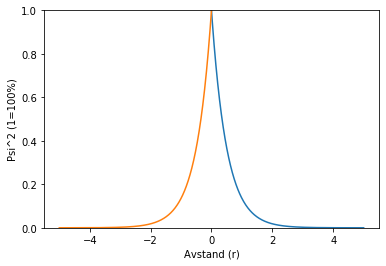
\includegraphics[scale=0.8]{plottbestemmegrenser.png}
\caption{Sannsynlighetsdistribusjon for bølgefunksjonen $\Psi(r_1r_2)=e^{-\alpha(r_1+r_2)}$. Grensene går mot 0, ved større avstand mellom elektronen.}
\label{fig: Grenser}
\end{figure}

\noindent Utifra figur 1 konvergerer grafen mot 0, grafen når $\approx$ når 0 når r ligger utenfor intervallet [-3,3]. Altså blir dette integrasjonsgrensene som brukes i Legendres metode.


\subsubsection{Gauss Kvadratur- Kartesiske Koordinater}
\noindent Koden som brukes til Legendre integrasjon er inspirert av eksempelkodene fra github[2].\\
\noindent Ved bruk av kartesiske koordinater holder det å bruke Legendres metode, med integrasjonsgrenser fra -3 til 3. Når det gjelder psudokoden kjøres Legendre funksjonen med de oppgitte grensene for å lage Legendrepolynomet. Videre er integranden lik det som ble oppgitt i oppgaveteksten. Denne integranden blir satt opp ved hjelp av en funksjon. Om avstanden mellom elektronene nærmer seg 0, vil funksjonen som lager uttrykket returnere 0 ved hjel av en if/else setning.\\
\noindent Videre vil dette uttrykket brukes i en seksdimensional for-loop for å regne ut vektene. Vektene blir videre brukt i samme loop ved å multiplisere disse med integranden som ble laget i starten.
\subsubsection{Gauss Laguerre- Sfæriske Koordinater}
\noindent Koden som brukes til Laguerre integrasjon er stort sett inspirert av eksempelkodene fra github[2].\\
\noindent Ved bruk av sfæriske koordinater er det som sagt tidligere i rapporten kun nødvendig å bruke laguerre på radialdelen, mens Legendre brukes på vinkelene på samme måte som med de kartesiske koordinatene, men med annerledes grenser naturligvis.

\noindent Psudokoden har store likheter som over, på samme måte, blir integranden produsert ved bruk av en funksjon. Også her returnerer funksjonen 0 om avstanden mellom elektronene blir for liten, ved hjelp av en if/else setning. Laguerrepolynomet produseres ved å kjøre radialdelen gjennom Laguerre funksjonen. Videre brukes en seksdimensional loop i dette tilfellet også. Den seksdimensionale loopen fungerer på samme måte som for Legendre over, bortsett fra at denne brukes på sfæriske koordinater. Koden kjøres og bruker legendre på vinklene og Laguerre på radialdelen som til slutt returnerer en approksimasjon til integralet.

\subsection{Monte Carlo metoden}
\noindent Koden og implementasjon av denne metoden er stor inspirert av eksemplene i Lecture Notes. Programmet starter med å definere de forskjellige variablene. Deretter blir det definert en vektor y som blir brukt til å lagre de tilfeldige tallene. Den aller viktigeste koden i dette programmet er nemlig løkken. Denne løkken starter med å finne tilfeldige tall mellom 0 og 1, ved bruk av funksjon $randu$, og disse blir lagret i x vektoren. Deretter blir x-vektoren brukt til å finne de andre variablene som inngår integranden. Så blir de variablene brukt til å rope integraden og dermed lagret i $fx$. $fx$ blir summert opp i $crude_m_c$ og kvadrat av $fx$ blir summert i $sum-sigma$. Deretter berenges integralet og variansen ved bruk av definisjonene ovenfor i teoridel.

\subsubsection{Brutekraft og uniform distribusjon}
\noindent Vektoren y blir fylt opp med verdier fra x vektoren ved bruk av ligning (9). Når alle disse verdiene har blitt lagret så blir de sendt funksjonen $integrate$. Denne funksjonen bruker disse innsendte variabelene til å regne ut $ledd1$ som er eksponentielle dellen av integranden og $ledd2$ som er nevneren. Og dette gjentas i løkken n-ganger.

\subsubsection{Forbedret MC og Importance sampling}
\noindent I denne metoden er det flere variabler å ta hensyn til.
$r_i$, $\cos(\theta)_i$ og $\phi_i$ blir regnet ved $x_i$-ene. Deretter så gjøres det samme som ovenfor. Disse sendes til funksjonen $ingerate-impor$ og her blir det regnet ut de forskjellige leddene i integranden. Dette gjøres n-ganger.

\section{Resultater}
\subsection{Gauss Kvadratur}
\noindent Resultatene fra Gauss kvadraturet kan ses i tabell 1.


\begin{table}[H]
\begin{tabular}{l|ll|ll}
\hline
N  & Svar-Legendre & Svar-Laguerre   & Relativ Feil-Legendre & Relativ Feil-Laguerre\\
\hline
10  & 0.0720 & 0.1865 & 0.6266 & 0.0327 \\
\hline
15  & 0.2391 & 0.1898 & 0.2403 & 0.0156\\
\hline
20  & 0.1561 & 0.1911 & 0.1900 & 0.0087\\
\hline
25  & 0.1958 & 0.1917 & 0.0158 & 0.0053 \\
\end{tabular}
\caption{Resultatene fra Gauss kvadraturet. N= antall integrasjonssteg, mens andre og tredje kolonne gir de approksimerte svarene til integralet. De to siste kolonnene gir relativ feil sammenliknet med det korrekte svaret: 0,1928.}
\end{table}

\noindent Plottet over de relative feilene mot N kan ses i figur 2.

\begin{figure}[H]
\centering
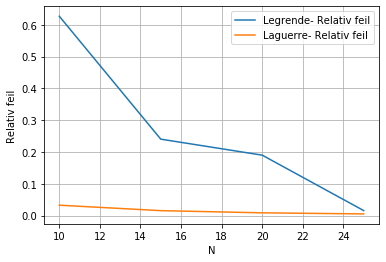
\includegraphics[scale=0.8]{resultatetgauskvadrat.png}
\caption{Relativ feil plottet for Legendre og Laguerre mot integrasjonssteglengde N. Feilene er de samme verdiene som fra tabell 1, men presentert på en annen måte da noen kan foretrekke plots fremfor grafer.}
\label{fig: Grenser}
\end{figure}

\subsection{Monte Carlo}
\begin{table}[H]
\begin{tabular}{l|ll|ll}
\hline
N  & I (Brute force) & I (Importance)  & Error (Brute force) & Error(Importance)\\
\hline
10e3  & 0.0720 & 0.1865 & 0.6266 & 0.0327 \\
\hline
10e4  & 0.2391 & 0.1898 & 0.2403 & 0.0156\\
\hline
10e5  & 0.1561 & 0.1911 & 0.1900 & 0.0087\\
\hline
10e4  & 0.1958 & 0.1917 & 0.0158 & 0.0053 \\
\end{tabular}
\caption{Resultatene fra Monte Carlo. N= antall integrasjonssteg, mens andre og tredje kolonne gir de approksimerte svarene til integralet. De to siste kolonnene gir relativ feil sammenliknet med det korrekte svaret: 0,1928.}
\end{table}

\begin{table}[H]
\begin{tabular}{l|ll|ll}
\hline
N  & V (Brute force) & V(Importance )  & Tid (Brute force) & Tid (Importance)\\
\hline
10e3  & 0.0720 & 0.1865 & 0.6266s & 0.0327s \\
\hline
10e4  & 0.2391 & 0.1898 & 0.2403s & 0.0156s\\
\hline
10e5  & 0.1561 & 0.1911 & 0.1900s & 0.0087s\\
\hline
10e4  & 0.1958 & 0.1917 & 0.0158s & 0.0053s \\
\end{tabular}
\caption{Resultatene fra Monte Carlo. N= antall integrasjonssteg, mens andre og tredje kolonne gir de approksimerte svarene til integralet beregnde verdiene til variansene. De to siste kolonnene gir CPU tiden for å kjøre algoritmen.}
\end{table}

\section{Diskusjon}
\noindent Ved bruk av Gauss-Legendres metode gir denne ut ifra tabell 1 for høy error ved bruk av lave N. Det er ikke før N nærmer seg 25 at metoden gir tilnærminger som er brukbare. Det positive er at ut ifra figur 2, synker den relative erroren ganske raskt med økende N.\\
\newline\noindent Når det gjelder Gauss-Laguerres metode synker feilen med økende N. Denne metoden gir også mye bedre approksimasjoner enn Legendre. Ved N=15 gir Laguerres metode tilsvarende relativ feil som Legendre hadde ved N=25.\\
\newline\noindent Her kan du fylle på mer
\section{Konklusjon}
\noindent Det er altså vist hvordan det er mulig å finne energien heliumatomet grunntilstanden ved bruk av forskjellige integrasjonsmetoder. Det ble vist at den parallelliserte Monte Carlo metoden er den best tilpassede metoden å velge til et slikt problem da denne både gir en gode approksimasjoner og er tidseffektiv. Det ble også vist at Gauss-Laguerre foretrekkes fremfor Gauss-Legendre da Laguerre gir bedre tilnærminger, samtidig som den er enkel å bruke ved integrasjonsgrenser som går mot \infty.

Konklusjonen er nesten ferdig men fint om du fyller på litt om montecarlo brute force og den andre for eksempel

\section{Appendiks}
\subsection{Omskrivning til sfæriske koordinater og "Laguerres form"}
\noindent For å skrive om til sfæriske koordinater tas det utgangspunkt i integralet som ble oppgitt, der $\alpha$=2.


\begin{equation}
\label{a}
A &= \int_{-\infty}^{\infty} dr_1dr_2 e^{-4(r_1+ r_2)} \frac{1}{\left| r_1 - r_2 \right|}
\end{equation}
\noindent Hvor $dr_1dr_2$= $r_1^2r_2^2 dr_1dr_2dcos(\theta_1)dcos(\theta_2)d\phi_1d\phi_2\\$ som igjen gir $dr_1dr_2$=$r_1^2r_2^2\sin\theta_1\sin\theta_2 dr_1dr_2d\theta_1d\theta_2d\phi_1d\phi_2$.\\

\noindent Dette føres i likning \ref{a} og gir:
\begin{equation}
   A= \int_{0}^\infty\int_0^\infty\int_0^{\pi}\int_0^\pi\int_0^{2\pi}\int_0^{2\pi}r_1^2r_2^2e^{-4r_1} e^{-4r_2} \sin\theta_1\sin\theta_2 dr_1dr_2d\theta_1d\theta_2d\phi_1d\phi_2
\end{equation}

\noindent Så gjøres uttrykket om ved å forandre variabler: $u_1 = 4r_1$ og $u_2 = 4r_2$, dette gir:

\begin{equation}
     A= \int_{0}^\infty\int_0^\infty\int_0^{\pi}\int_0^\pi\int_0^{2\pi}\int_0^{2\pi} \frac{1}{(2\alpha)^5}\intlimits u_1^2u_2^2e^{-u_1}e^{-u_2} \frac{\sin\theta_1\sin\theta_2}{\sqrt{u_1^2 + u_2^2 - 2u_1r_2\cos\beta}} du_1du_2d\theta_1d\theta_2d\phi_1d\phi_2\\
\end{equation}

\noindent Som gir integralet vårt på "Laguerres form"
\begin{equation}
 A=\frac{1}{(2\alpha)^5} \int_{0}^\infty\int_0^\infty\int_0^{\pi}\int_0^\pi\int_0^{2\pi}\int_0^{2\pi}W(u_1)W(u_2)g(u, \theta, \phi)\,du_1du_2d\theta_1d\theta_2d\phi_1d\phi_2.
\end{equation}


\section{Bibliografi}
\noindent [1] Morten Hjorth-Jensen, august 2015, Computational Physics Lecture Notes, 7 Eigensystems,
(https://github.com/CompPhysics/ComputationalPhysics/
blob/master/doc/Lectures/lectures2015.pdf)\newline

\noindent [2] Morten Hjorth-Jensen, 2019, Codeexamples,\newline
(https://github.com/CompPhysics/ComputationalPhysics/tree/master/doc/Projects/2019/Project3/CodeExamples)\newline

\noindent [3] Morten Hjorth-Jensen, september 2019 Project 3,\newline https://github.com/CompPhysics/ComputationalPhysics/blob/master/doc/Projects\newline
/2019/Project3/pdf/Project3.pdf.\newline


\noindent Link til githubmappen: https://github.com/philipkarim/Philip-and-Rohullah-ComFys




% ------------------- end of main content ---------------

\end{document}
